\chapter{Revisão Bibliográfica} \label{chap:sota}



\section{\ecat}\label{sec:ethercat}

A rede \ecat é uma rede de \emph{Ethernet} industrial que usa a
especificação padrão IEEE 802.3 \cite[]{ieee:IEEEStandardEthernet} para
definir o formato dos \emph{frames} e camada física a utilizar, mas
introduz uma maneira diferente de os processar.

Esta nova forma de processamento permite uma comunicação com todos os
dispositivos presentes na rede com apenas um \emph{frame}. \ecat utiliza
uma tipologia de comunicação \emph{Master/Slave}, tipicamente implementada
em formato \emph{daisy-chain}. 

Apenas o dispositivo mestre pode iniciar um \emph{frame} de comunicação
e os dispositivos escravos limitam-se a ler a parte informação contida
no \emph{frame} que lhes é endereçada. Ao mesmo tempo, cada dispositivo
escravo pode introduzir informação sua  no \emph{frame} antes de o enviar
para o dispositivo seguinte.

Estas caraterísticas permitem que o dispositivo mestre seja implementado
em qualquer tipo de dispositivo que contenha uma porta de comunicação 
\emph{Ethernet}. Os dispositivos escravo utilizam um \emph{EtherCAT Slave
Controller} (ESC) que processa os \emph{frames} fazendo com que a velocidade
e tempos de resposta da rede sejam previsíveis e independentes dos 
dispositivos escravo que existam na rede.


\section{Definição e caraterização do problema}\label{sec:problem}




\section{Soluções propostas} \label{sec:solution}

Para atingir os objetivos propostos por esta dissertação, foram propostas 
duas possíveis soluções. Ambas são apresentadas de seguida sendo que
maior ênfase será dada na última, pois é a proposta que se mostra mais
adequada ao estudo em questão.

No entanto, em qualquer uma das implementações existe uma ideia base
relativa à arquitetura da rede \ecat que se pretende implementar,
mostrada na figura \ref{fig:network-architecture}, fazendo-se uso da
tipologia \emph{daisy-chain}.

\begin{figure}
 \centering
 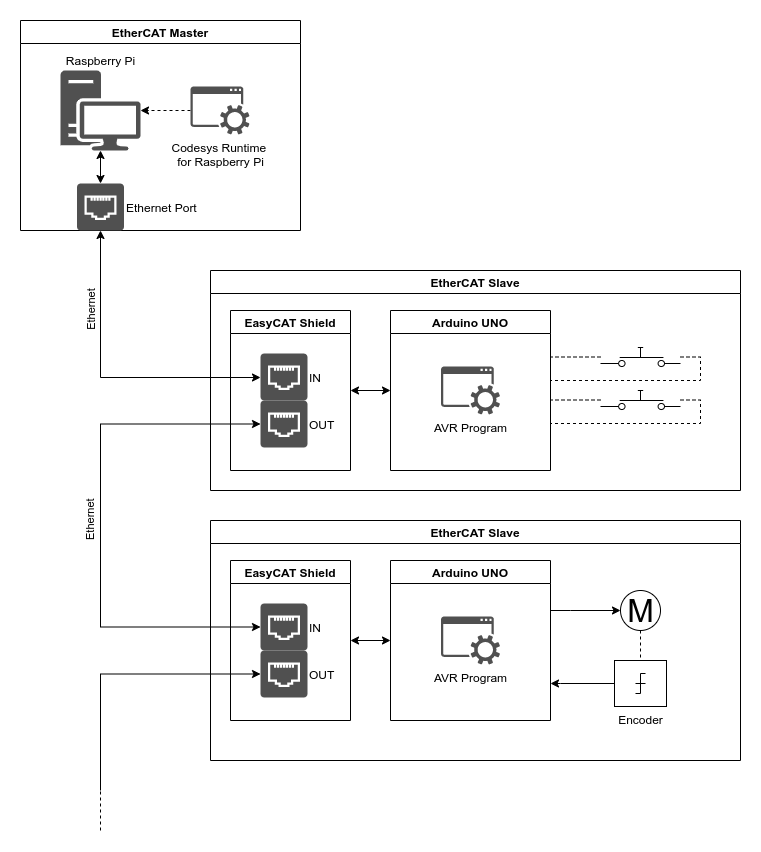
\includegraphics[width=0.75\linewidth]{network-diagram_transparent.png}
 \caption{Arquitetura da rede \ecat pretendida}
 \label{fig:network-architecture}
\end{figure}



\subsection{Controlo de discos perfurados}

A primeira solução idealizada no contexto desta dissertação foi o 
desenvolvimento de um sistema fisicamente simples, capaz de demonstrar
as capacidades de resposta temporal e sincronização de relógios de uma
rede \ecat.

Esta proposta baseia-se num sistema constituído por discos perfurados
na sua extremidade, acoplados a motores rotativos independentes. Por sua
vez estes motores serão controlados por módulos \emph{slave} \ecat
produzidos através de um Arduino UNO \cite[]{arduino:ArduinoUNORev3} e 
um \emph{shield EasyCAT} da \cite{ABT:EasyCAT}.

\subsection{Seguimento de um traçado com um braço robótico}


